% IEEE ISPA 2026 full regular paper.
\documentclass[conference]{IEEEtran}
\IEEEoverridecommandlockouts
\usepackage[T1]{fontenc}
\usepackage{cite,amsmath,amssymb,graphicx,booktabs,array,url,balance,needspace}
\usepackage{algorithm,algorithmic}
\begin{document}
\title{Interface-Closed Recovery: Joint Workflow Repair with Observed-Input Certificates}
\author{%
\IEEEauthorblockN{1\textsuperscript{st} Zhengyuan Dai}
\IEEEauthorblockA{\textit{Southwest University}\\
Chongqing, China\\
Zhengyuan-Dai@outlook.com}
\and
\IEEEauthorblockN{2\textsuperscript{nd} Yuhang Zou}
\IEEEauthorblockA{\textit{Southwest University}\\
Chongqing, China\\
zyh18769362802@email.swu.edu.cn}
\and
\IEEEauthorblockN{3\textsuperscript{rd} Yuming Fu}
\IEEEauthorblockA{\textit{Southwest University}\\
Chongqing, China\\
fym10276612@email.swu.edu.cn}
\and
\IEEEauthorblockN{4\textsuperscript{th} Bo Liu\textsuperscript{*}}
\IEEEauthorblockA{\textit{Southwest University}\\
Chongqing, China\\
liubocq@swu.edu.cn}
\thanks{\textsuperscript{*}Corresponding author: Bo Liu}}
\maketitle
\begin{abstract}
When a tool in a language-model agent fails, replacing one call can break
downstream interfaces or change a value needed by the remaining workflow. We
present Interface-Closed Recovery (ICR), which jointly chooses replacements
and the least changed region that reconnects to unchanged execution. Its
recovery packet carries interface, function, and boundary-value evidence. On
a fixed read-only relation, functional dependencies and a common-row witness
certify paths at the observed input without executing them. Across 1,901
TaskBench graphs, ICR's exact solver matches exhaustive search and finds 484
repairs missed by matched-information greedy. On PlanBench-XL, the certificate
recovers 774 additional safe shortest-route decisions over global certification
and avoids 126 incorrect type-only choices across 9,250 failed-tool--input
cases. An executor-backed replay confirms that joint repair preserves unchanged
downstream calls. In a sealed 72-task study, the complete ICR advice system
passes 58 tasks versus 39 for the native agent. At 20 matched input-only
failure prefixes, it restores the trusted target value within 12 turns in 19
cases versus seven for global-certificate advice.

\end{abstract}
\begin{IEEEkeywords}
language-model agents, workflow recovery, interface contracts, program synthesis
\end{IEEEkeywords}

\section{Introduction}
Language-model agents must recover from failed tools while preserving the
remaining workflow. Interleaved reasoning and action~\cite{react} leaves
dependency repair to local model decisions.

Replacing one call can break its consumer; replacing the entire suffix discards
valid work. Recovery must choose where to reconnect and preserve the failed
operation's boundary value at the observed input. Interface connectivity alone
cannot establish value preservation.

We introduce Interface-Closed Recovery (ICR) and make three contributions.
First, we define joint implementation-and-scope repair with a least
reconnection boundary and exact structural solvers for forests and bounded-width
port-bound directed acyclic graphs (DAGs). Second, a recovery packet combines
function eligibility, validated context, observed-value binding, and a
boundary-value certificate. On a fixed relation under trusted tool contracts,
dependency and row-support evidence admits input-specific paths without
executing candidates; separate policies govern advice and dispatch. Third,
TaskBench tests structural exactness, an executor replay tests combined scope
and value admission, and PlanBench-XL supplies sealed 72-task and 20-prefix
native-agent comparisons.
ICR is available at \url{https://github.com/zhengyuancode/ICR}.

\section{Motivation and Problem Formulation}
\subsection{Why Local Substitution Fails}
A mesh snapshot feeds a mesh-specific publisher. If the snapshot tool fails,
an alternative producer may return a bridge payload for the same device.
Replacing only the producer breaks the consumer interface; replacing both can
preserve the output boundary and resume the unchanged continuation
(Fig.~\ref{fig:continuation-workflow}). The stopping point is therefore part of
the recovery decision. We write $f$ for the failed producer, $c$ for its
catalog-linked consumer, and $i,o$ for the immutable input and output ports.
For a fixed replacement assignment $\rho$, $R^*_{\rho}$ is its least
interface-closed repair region. A failure record $\xi$ contains the observed
failed input $a$, and $\mathcal{P}(\xi)$ denotes the compiled interface-closed
program set available at that failure.

The formal model covers an acyclic explicit dataflow. A port contract is a
predicate over explicit inputs, outputs, and failure outcomes. In the evaluated
read-only setting, an observable effect is the normalized value returned at an
immutable boundary; state-changing calls already committed to an external
system belong to $M$ and are never replaced. Online task completion is an
empirical endpoint rather than a consequence of the dataflow theorem.

ICR separates scope, compatibility, function, observed-value binding, and
input-conditional value preservation. Its packet carries the program, context,
and evidence; dispatch remains a separate authority decision.

\begin{figure*}[t]
\centering
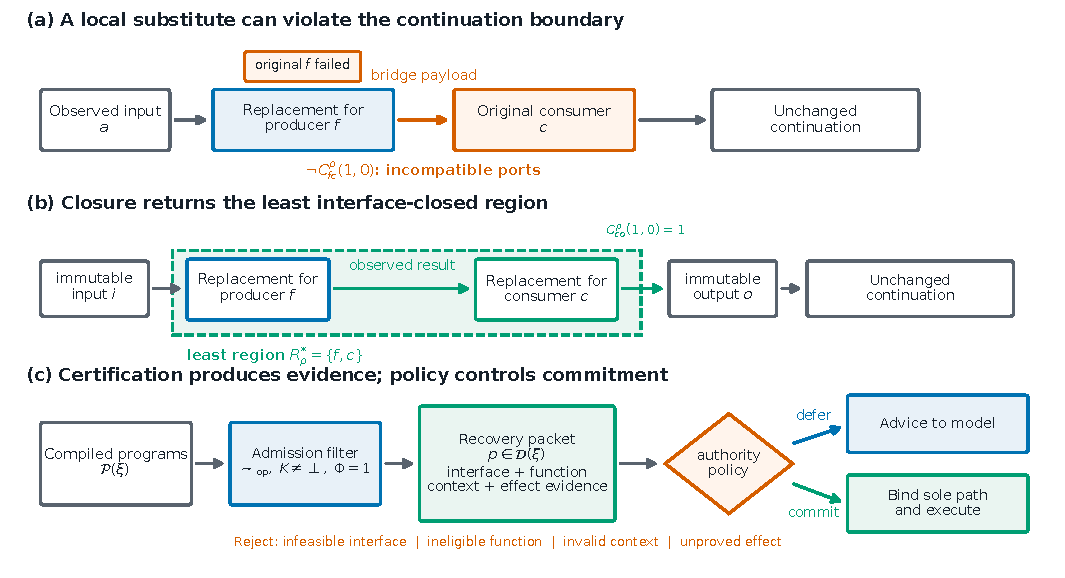
\includegraphics[width=.96\textwidth]{figures/continuation_workflow.pdf}
\caption{Interface-closed recovery from local substitution to a certified,
policy-gated continuation.}
\label{fig:continuation-workflow}
\end{figure*}

\subsection{Interface-Closed Region}
Let $G=(V,E)$ be an interface-valid workflow, $F\subseteq V$ the failed
required nodes, and $M\subseteq V$ the immutable nodes, including committed
effects and external ports. For a fixed candidate assignment $\rho$, each node
has its original or replacement implementation. For $(u,v)\in E$, let
$C^{\rho}_{uv}(b_u,b_v)$ indicate compatibility of the selected ports when
$b_u,b_v\in\{0,1\}$ choose the original implementation or the replacement
specified by $\rho$. The original graph satisfies $C^{\rho}_{uv}(0,0)$.

A repair region $R$ is feasible for $\rho$ if
\begin{equation}
 F\subseteq R\qquad R\cap M=\varnothing\qquad
 \bigwedge_{(u,v)\in E}C^{\rho}_{uv}(\mathbf{1}_{u\in R},\mathbf{1}_{v\in R})
 \label{eq:region-feasibility}
\end{equation}
The structural objective minimizes nonnegative node-change cost. Immutable
external ports preserve the unchanged interface. The least feasible region
under $\rho$ induces program $p_{\rho}$.
Let $\Phi(p_{\rho},a)$ denote boundary-value eligibility at the observed input and
$K(p_{\rho},\xi)$ the validated context, with $K(p_{\rho},\xi)=\bot$ on
validation failure. Structural closure enforces~\eqref{eq:region-feasibility};
admission also requires $\Phi(p_{\rho},a)=1$ and $K(p_{\rho},\xi)\ne\bot$.


\section{Interface-Closed Recovery}
\label{sec:interface-repair}
\subsection{Bidirectional Repair Closure}
A replacement propagates two kinds of obligations. If its output is
incompatible with an unchanged consumer, that consumer must enter the region.
Conversely, a replaced consumer may reject an unchanged predecessor's output,
requiring that predecessor to enter. Construct the implication relation
\begin{equation}
\begin{split}
 u\Rightarrow v &\quad\text{if }(u,v)\in E\land\neg C^{\rho}_{uv}(1,0)\\
 v\Rightarrow u &\quad\text{if }(u,v)\in E\land\neg C^{\rho}_{uv}(0,1)
\end{split}
\end{equation}
Starting with $R_0=F$, compute
\begin{equation}
 R_{k+1}=R_k\cup\{v:\exists u\in R_k,\ u\Rightarrow v\}
 \label{eq:repair-closure}
\end{equation}
This inflationary monotone operator reaches a fixed point $R^*_{\rho}$ on a finite
graph. The worklist records the implication responsible for every added node,
providing a checkable explanation of the repair region.
Figure~\ref{fig:repair-obligations} illustrates both propagation directions
and an immutable-boundary conflict.

\begin{figure}[t]
\centering
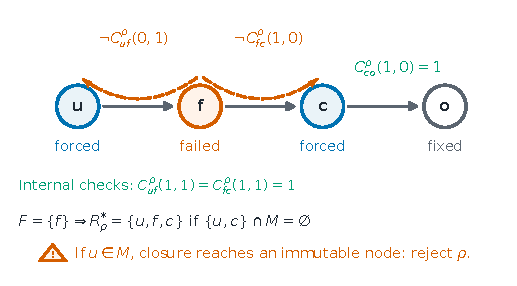
\includegraphics[width=\columnwidth]{figures/repair_obligations.pdf}
\caption{Bidirectional closure and feasibility checks.}
\label{fig:repair-obligations}
\end{figure}

\textbf{Theorem 1 (least feasible region).}
For a fixed replacement assignment $\rho$ and its Boolean compatibility relation, if
$R^*_{\rho}\cap M=\varnothing$ and every edge $(u,v)$ internal to $R^*_{\rho}$ satisfies
$C^{\rho}_{uv}(1,1)$,
then $R^*_{\rho}$ is the unique inclusion-least feasible region. Otherwise no feasible
region exists for that assignment.

Every feasible region contains $F$ and is closed under each forced implication,
so it contains $R^*_{\rho}$. Edges $(u,v)$ with both endpoints outside retain
$C^{\rho}_{uv}(0,0)$; closure checks
mixed edges, and the final test checks internal edges.

It follows that $R^*_{\rho}$ minimizes any nonnegative additive node-change cost for
the fixed assignment. A worklist examines each node once and each edge at most
twice, taking $O(|V|+|E|)$ time after compatibility is available. Enumerating a
finite assignment set $\mathcal{A}$ and choosing its smallest feasible closure
is exact over $\mathcal{A}$; the cost of discovering that set is separate.

\textbf{Theorem 2 (contextual interface preservation).}
When compatibility predicates are sound for the port contracts, replacing
exactly the nodes of a feasible $R^*_{\rho}$ preserves all interfaces of the unchanged
context. Consider an acyclic workflow whose tools are deterministic functions
of their explicit inputs, share no hidden mutable state, honor the same declared
failure semantics, and execute unchanged nodes in their original topological
order. The resulting dataflow remains well typed. If the replacement also
preserves every normalized value exposed at the repair boundary, the unchanged
continuation produces the same observable suffix outputs.

Every edge is original--original, mixed, or replacement--replacement;
the original contract, closure, or final test checks each case, respectively.
Topological induction then propagates valid types, and matching exposed
values preserves the deterministic suffix.

These properties identify when single-call substitution is insufficient:
if $\neg C^{\rho}_{fc}(1,0)$, every feasible repair containing the failed producer
$f$ must also include consumer $c$. The boundary, rather than a fixed repair
depth, determines where repair may stop. The guarantees concern interface
composition; functional eligibility must be supplied separately.

\subsection{Joint Choice and Scope}
Fixed-assignment closure does not select implementations. Let $A_v$ contain
node $v$'s original $0_v$ and operation-equivalent alternatives; eligibility
is checked before interface optimization. Let $c_v(s)\geq0$ be choice cost,
$c_v(0_v)=0$, and $\Gamma_{uv}(s,t)$ denote edge compatibility.
The joint decision is
\begin{equation}
\begin{split}
\min_{x_v\in A_v}\quad &\sum_{v\in V}c_v(x_v)\\
\text{s.t.}\quad &x_f\ne0_f\ (f\in F)\quad x_m=0_m\ (m\in M)\\
&\Gamma_{uv}(x_u,x_v)=1\quad((u,v)\in E)
\end{split}\label{eq:joint-choice}
\end{equation}
Source and sink ports remain immutable. Assignment $\vec{x}=(x_v)$ changes
region $R(\vec{x})=\{v:x_v\ne0_v\}$; the cheapest seed need not minimize
total repair cost. Theorems~3 and~4 solve this structural objective; context
and value admission then filter the resulting programs.

For a forest, root each underlying undirected component arbitrarily. For a
tree parent $v$ and child $w$, let $B_{vw}(s,t)=\Gamma_{vw}(s,t)$ when
$(v,w)\in E$, and $B_{vw}(s,t)=\Gamma_{wv}(t,s)$ otherwise. Thus $B$ always
orders its arguments as parent then child while preserving dataflow direction.
Let $D_v(s)$ be the minimum cost of the subtree below $v$ conditional on
$x_v=s$. For child $w$,
\begin{equation}
D_v(s)=c_v(s)+\sum_{w\in\mathrm{ch}(v)}
\min_{t\in A_w:\,B_{vw}(s,t)=1}D_w(t)
\label{eq:joint-dp}
\end{equation}
where an empty minimum is $+\infty$. Ineligible choices have infinite cost. Backtracking
from the minimum root state returns both selected implementations and
$R(\vec{x})$.

\textbf{Theorem 3 (exact joint repair on forests).}
Equation~\eqref{eq:joint-dp} returns a globally minimum-cost assignment
satisfying~\eqref{eq:joint-choice}, or reports infeasibility. With $k_v=|A_v|$,
it takes $O(\sum_{(u,v)\in E}k_uk_v+\sum_v k_v)$ time and
$O(\sum_v k_v)$ score states; storing backpointers additionally uses
$O(\sum_{(v,w):w\in\mathrm{ch}(v)}k_v)$ memory.

\emph{Proof.} Conditional on $x_v=s$, child subtrees are independent;
leaf-to-root induction makes $D_v(s)$ their optimum. Minimizing each root
gives the global optimum or infeasibility. Edge option pairs and states give
the stated bounds.\hfill$\square$

Algorithm~\ref{alg:joint-repair} summarizes the exact forest procedure and its
returned assignment and region.

\begin{algorithm}[!b]
\caption{\textsc{ExactJointRepair} on a forest}
\label{alg:joint-repair}
\footnotesize
\begin{algorithmic}[1]
\REQUIRE Rooted forest $G$; choices $\{A_v\}$; costs $\{c_v\}$;
compatibility $\Gamma$; failed nodes $F$; immutable nodes $M$
\ENSURE Minimum-cost $(\vec{x}^{*},R(\vec{x}^{*}))$, or
\textsc{infeasible}
\STATE Remove original choices at failed nodes and nonoriginal choices at
immutable nodes
\STATE Remove choices that violate immutable source or sink ports
\STATE For each $v$ in postorder and $s\in A_v$, compute $D_v(s)$
by~\eqref{eq:joint-dp}
\IF{some root has no finite state}
  \RETURN \textsc{infeasible}
\ENDIF
\STATE Backtrack the minimizing states
\RETURN $(\vec{x}^{*},R(\vec{x}^{*}))$
\end{algorithmic}
\end{algorithm}

For multi-input DAGs, port-bound edges yield pairwise compatibility factors.
Min-sum variable elimination~\cite{dechter1999bucket} with min-fill ordering
and backpointers extends exact repair to shared consumers.

\textbf{Theorem 4 (bounded-width joint repair).}
For a port-bound workflow whose induced elimination width is $w$ and whose
nodes have at most $k$ eligible implementations, min-sum variable elimination
solves~\eqref{eq:joint-choice} exactly in
$O((|V|+|E|)k^{w+1})$ time and
$O(|V|k^w+|E|k^2)$ memory including the original pairwise factors,
or reports infeasibility.
Elimination preserves separator optima; temporary factors have at most $w+1$
variables, and backtracking attains the optimum. Forests have width one.

With arbitrary supplied pairwise compatibility predicates, deciding whether
any joint repair exists is nondeterministic polynomial-time (NP)-complete even when the dependency graph is a
DAG and each failed node has only three eligible replacements: orient a
3-coloring instance acyclically and make adjacent replacement colors
incompatible. Bounded width therefore gives a tractable exact class.


\subsection{Compiling Local Recovery Programs}
The compiler constructs a local graph $i\to f\to c\to o$, where $f$ is the
failed producer, $c$ a catalog-linked continuation, and $i,o$ immutable input
and output ports. For each alternative producer and consumer in the same
respective public categories and domains, it constructs a compatibility table
and invokes the fixed-point closure with $F=\{f\}$ and $M=\{i,o\}$. Enumeration includes
the original consumer and does not prefilter on internal or output-boundary
compatibility. Closure therefore determines whether to retain $c$, replace
it, or reject the assignment.

Three evidence tests instantiate this table. The input edge requires a
lossless transport of the observed failed-call arguments. The internal edge
uses nominal producer references and a unique payload projection for each
old--new combination. The output edge requires the chosen consumer's
normalized public output schema to equal the original boundary. The compiler
stores every forced inclusion and rejection alongside the emitted program.
It emits only the nodes chosen by closure as replacements; an unchanged
consumer can still execute as the continuation.

\textbf{Corollary (local structural admission).}
If the alternative producer cannot bind to the original consumer, then a
candidate is structurally admitted exactly when concrete input transport, alternative-pair
binding, and output-boundary preservation all hold. Its least region is
$\{f,c\}$. Otherwise, a valid input transport admits the producer-only region
$\{f\}$ with the original consumer. Function, context, and boundary-value gates are
applied after this structural test.

With $f$ forced and the ports immutable, an incompatible original consumer
forces $c$ into the region. The three evidence tests then check precisely its
input, internal, and output boundaries.

Theorem~1 applies exactly to this Boolean structural relation. Nominal
annotations establish payload identity for interface checking; the separate
boundary-value predicate establishes semantic eligibility. Concrete input validation
checks the selected dataflow at execution time. Theorem~2 gives the typing
guarantee under sound application port contracts.

Each candidate exposes a function whose arguments contain only the context
still needed from the model. After selection, the executor invokes the
producer, binds its actual successful output into the consumer, validates
the resulting input, and invokes the consumer. A failed producer interrupts
the program before the consumer is dispatched. The original failure and both
recovery invocations remain in the execution trace. This separates semantic
choice from deterministic dataflow binding.

\subsection{Recovery Packet and Authority Boundary}
At an observed failure record $\xi$ containing failed input $a$, let
$\mathcal{P}(\xi)$ be the locally compiled interface-closed programs. A declared
operation relation $\sim_{\mathrm{op}}$ admits a
replacement only when its producer and consumer retain the respective
operations of the failed call and intended continuation. In the relational
instantiation, this requires the same source--target projection signature;
$\Phi$ below supplies the input-specific value evidence. At program level,
$K(p,\xi)$ returns context assembled from
observed arguments, public defaults, and explicit task fields, and
$K(p,\xi)=\bot$ when that context does not validate against the program's public
input schema. The boundary-value predicate $\Phi(p,a)$ accepts a program only
when its returned value is certified at the observed input. The dispatch set is
\begin{equation}
\begin{aligned}
\mathcal{D}(\xi)=\{p\in\mathcal{P}(\xi):\;&
p\sim_{\mathrm{op}}\xi\ \land\ K(p,\xi)\ne\bot\\
&{}\land\ \Phi(p,a)=1\}
\end{aligned}
\label{eq:dispatch-set}
\end{equation}
The recovery packet records an admitted program, its validated inputs,
interface boundary, and boundary-value evidence. The advice policy returns the packet
to the model; the dispatch policy executes the sole member when
$|\mathcal{D}(\xi)|=1$ and otherwise returns the candidates. Context extraction copies matching failed-call arguments, uses
public schema defaults, and recognizes explicit priority or channel in the
user request. It never reads benchmark reference paths or judge labels.

\textbf{Proposition (choice collapse).} Conditional on a sound operation
relation, sound interface and boundary-value predicates, valid context, and a non-committing failed
call, if $\mathcal{D}(\xi)=\{p\}$, every recovery restricted to the declared
operation-equivalent, context-valid, value-certified local program class
selects $p$. Executing $p$
preserves the unchanged dataflow boundary; its consumer receives a projection
of the observed producer result, not a predicted value.

Within the declared local class, this rule removes a determined choice from
the model's action space; ambiguous or uncertified recovery remains with the
model. The certificate establishes local execution admissibility, while eager
dispatch is an authority policy that changes the agent's subsequent history.
The online advice control exposes the same certificate and context but leaves
selection and execution to the model.

\textbf{Observed-input certificate.} A global boundary-value certificate can
reject a route that is valid for the failed call's actual input: a sparse
intermediate attribute may be absent elsewhere but present on the observed
row. Let $\pi=(X_0,\ldots,X_\ell)$ replace a unary projection from $X_0$ to
$X_\ell$ over relation $T$ at observed input $a$, where the unblocked
original is defined. We require functional
dependencies $X_0\to X_\ell$ and $X_{j-1}\to X_j$ for every path edge, plus
\begin{equation}
 \exists r\in T:\ r[X_0]=a\ \land\ \bigwedge_{j=0}^{\ell}r[X_j]\ne\mathrm{NULL}
 \label{eq:input-support}
\end{equation}
Here $\mathrm{NULL}$ is a missing database cell, distinct from a tool exception
or failed invocation. Values are compared after the benchmark executor's public
normalization; lossy or nonunique conversions do not satisfy $\Phi$. The row witnesses a defined route; the dependencies make every edge
single-valued. Induction proves that $\pi(a)$ equals the failed tool's result
without executing $\pi$. This specializes database dependencies and conditional
equivalence~\cite{abiteboul1995foundations,kawaguchi2010conditional} to a
failure-time gate. The guarantee is conditional on the declared projection
semantics, the functional dependencies holding on $T$, and an unchanged
snapshot during lookup and execution. A trusted backend compiler checks these
conditions and precomputes witness memberships; runtime admission is an indexed
lookup with no candidate execution or model call. The online study compares
this gate with global certification and type-only admission.

\begin{figure}[t]
\centering
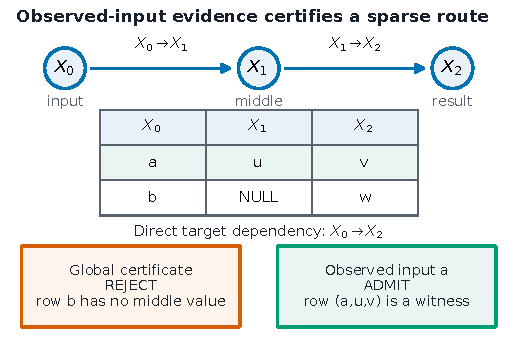
\includegraphics[width=\columnwidth]{figures/input_index_certificate_adjusted.pdf}
\caption{Observed-input certification of a globally rejected relational route.}
\label{fig:input-index-certificate}
\end{figure}


\section{Experimental Methodology}
\subsection{Implementation}
ICR observes the public tool catalog, concrete call arguments, returned
observations, and an append-only execution ledger. It never receives benchmark
injection labels, reference paths, task solutions, or judge verdicts. Tool
definitions supply input schemas, output annotations, categories, domains,
and declared substitutes. We retain PlanBench-XL's native retail
executor~\cite{planbenchxl}.

ICR separates a trusted backend compiler from the end-user agent. In the
PlanBench-XL deployment, the compiler may read the benchmark's released,
fixed retail relation to build a certificate index; neither ICR's language
model nor the native-agent control can inspect relation rows. Global,
observed-input, and type-only advice controls use the same compiler-side
catalog and index. Native-versus-ICR results therefore evaluate the deployed
recovery system, while matched advice controls isolate admission policy.

After an observed failure, the compiler enumerates alternative producers and
linked consumers, constructs their compatibility table, and computes the least
repair region. Admission requires lossless transport of supplied producer
arguments, a unique projection that binds the observed payload into the
consumer, and preservation of the original output schema. Generic
``data'' or ``object'' matches are rejected. At execution, a failed producer
interrupts the program before its consumer is dispatched; the original
failure and all recovery calls remain in the trace.

Candidate generation does not assume that a new failure is permanent. An
identical-call retry gate permits one further attempt unless persistence is
explicit; declared direct substitutions retain precedence when their concrete
inputs validate. Every matched online control uses the same catalog, retry
rule, retriever, executor, and failure trigger.

\subsection{Studies and Controls}
We evaluate structural optimality, boundary-value safety, and
online completion separately. Within each comparison, controls receive the
same frozen unit, public catalog, model, executor, and limits; reference paths
and judge labels enter only offline scoring.

\textbf{RQ1: structural exactness and joint choice.}
An exhaustive small-graph suite covers 40,824 fixed-assignment instances;
runtime audits enumerate all 16 regions of every recorded local assignment.
A local processor probe uses worst-propagation chains up to 50,000 nodes.
The multi-node study deduplicates 1,901 one-input TaskBench Multimedia and
Hugging Face graphs~\cite{taskbench}; each failed node receives 128 seeded
domain replacements, type equality defines compatibility, and external ports
remain immutable. Distinct graphs are cluster-bootstrapped and two additional
assignment seeds check stability.

For joint choice, every published operation receives two controlled format
variants from plain text, JSON, and protobuf, with fixed sampled costs and
unchanged operation identity. Exact DP, matched-information greedy, beam
controls, and the exhaustive oracle receive identical choices, boundaries,
costs, and compatibility tables. On 157 additional multi-input DAGs, variable
elimination and beams receive the same port-bound variants. Four-choice and
additional-seed runs test sensitivity. These interventions isolate interface
optimization; the executable catalog in RQ2 tests boundary-value effects.

\textbf{RQ2: boundary-value admission and native-agent recovery.}
PlanBench-XL supplies 327 retail queries, 185 typed tools, and a released
100-row read-only relation. Without reading task solutions, we enumerate
boundary-compatible paths of at most five calls. For the relational
certificate, all 136 unary edge dependencies are checked exhaustively on the
fixed relation; this is a finite-snapshot guarantee, not an inference about
future data. The compiler then indexes non-null row witnesses. Compilation
takes 0.172\,s and no tool or model calls. The index occupies 2.36\,MiB on disk
and 6.23\,MiB when parsed; 9,850 hash-and-lookup probes take a median
1.72\,$\mu$s each on one processor. Exhaustive native replay is used
only after compilation to audit all 31,565 path--input classifications. A
separate calibration/held-out replay rule provides an empirical comparator.

The online policies are native execution, type-only advice,
global-certificate advice, and ICR advice using the observed-input certificate.
A 29-prefix development study precedes an all-arm, reserved 21-task seed-42
holdout. The target population is explicit-blocker tasks with at least one
available globally certified local bypass, defined before model outcomes. Of 134 tasks untouched by
earlier development, 102 met this structural rule (76.1\%). Under seed 43 these
102 eligible tasks were frozen;
the first 30 served as diagnostics and the remaining 72 formed the sealed
independent-task confirmation. A separate 80-task schedule captures previously
unused input-only opportunities. Six prefixes form a pilot; the next 20 form
the sealed same-prefix comparison, with identical histories, states, and
failed actions. Its predeclared primary endpoint is restoration of the trusted
target value within 12 subsequent model turns; whole-task success is
secondary. An ancillary post-primary type-only arm replays the same 20
prefixes. Table~\ref{tab:study-map} separates their estimands and units.

\begin{table*}[t]
\centering\footnotesize\setlength{\tabcolsep}{5pt}
\caption{Evaluation cohorts and primary estimands.}
\label{tab:study-map}
\begin{tabular}{llll}
\toprule
\textbf{Study} & \textbf{Unit} & \textbf{Comparison} & \textbf{Primary endpoint}\\
\midrule
Structural oracle & 6,975 node failures in 1,901 graphs & DP, greedy, beams, oracle & Feasibility and minimum cost\\
Static certificate & 31,565 path--input pairs & Global, type only, observed input & Native-executor value equality\\
System confirmation & 72 globally certified-bypass tasks & Native vs. complete ICR advice & Whole-task completion\\
Admission holdout & 21 reserved tasks & Three certificate policies & Whole-task completion\\
Same-prefix confirmation & 20 input-only failure states & Three certificate policies & Target restoration within 12 turns\\
\bottomrule
\end{tabular}
\end{table*}

\subsection{Online Settings and Statistics}
All online arms use the same hosted endpoint, which reports the served-model
identifier \texttt{deepseek-flash}.
Temperature is zero, thinking is disabled, and the response cap is 4,096
tokens. PlanBench-XL retains its 100-step cap.
We use 100,000 paired template, task, or prefix bootstrap resamples (seed
20260924); reported 95\% intervals are percentile intervals. TaskBench graph
resamples are stratified by domain. Exact paired binary tests use the two-sided
McNemar test. The sealed 72-task and 20-prefix studies use task and matched
prefix as their respective units; pilots and ancillary controls are not pooled
with them. Every paired 72-task run reached a terminal benchmark outcome; no
task was omitted because of a missing model response.

\section{Results}
\subsection{Structural Recovery and Joint Choice}
The multi-node TaskBench study evaluates 892,800 fixed assignments on 1,901
distinct Multimedia and Hugging Face graphs. Among 28,933 feasible cases
whose replacement changes an adjacent interface, the least fixed point
matches an exhaustive subset oracle in every case. One and two rounds of
otherwise identical implication propagation miss 3,338 and 218 repairs,
respectively. The one-round recall gap is 11.5 percentage points (graph-bootstrap 95\%
interval [10.8, 12.3]); both extra assignment seeds give similar gaps.
A 50,000-node chain closes in 73.7\,ms median on one processor.

Each graph contributes one instance per possible failed node, giving 6,975
instances. All methods in Table~\ref{tab:joint-choice} receive identical candidates,
costs, immutable boundaries, and compatibility tables. ``Oracle match''
requires the same feasibility status and, when feasible, the same minimum cost.
\begin{table}[t]\centering\small\setlength{\tabcolsep}{4pt}
\caption{Joint repair on 1,901 TaskBench topologies.}
\label{tab:joint-choice}
\begin{tabular}{ccc}\toprule
\textbf{Method} & \textbf{Repairs found} & \textbf{Oracle match}\\\midrule
Forward greedy & 3,449/6,975 & 6,472/6,975\\
Beam width 2 & 3,745/6,975 & 6,786/6,975\\
Beam width 4 & 3,914/6,975 & 6,956/6,975\\
Beam width 8 & \textbf{3,933/6,975} & \textbf{6,975/6,975}\\
ICR joint tree DP & \textbf{3,933/6,975} & \textbf{6,975/6,975}\\
\bottomrule\end{tabular}\end{table}

Joint tree DP finds 484 feasible repairs missed by the matched-information
forward greedy rule, a gain of 6.9 percentage points (graph-bootstrap 95\% interval
[6.3, 7.6]); width-four beam misses 19. On 157 multi-input DAGs, exact
elimination matches the oracle at every one of 568 oracle-checkable positions.
With four implementations per operation, width-eight beams miss one to four
feasible DAG repairs across three independent seeds; elimination remains exact.
On three-choice chains, the exact DP scales from 0.040\,ms at three nodes to
117.4\,ms at 10,000 nodes, whereas exhaustive enumeration already takes
51.6\,ms at 11 nodes.
The graph experiments preserve each published operation's identity while
varying declared interface formats, isolating repair-scope optimization from
language-model generation.

\begin{figure*}[t]
\centering
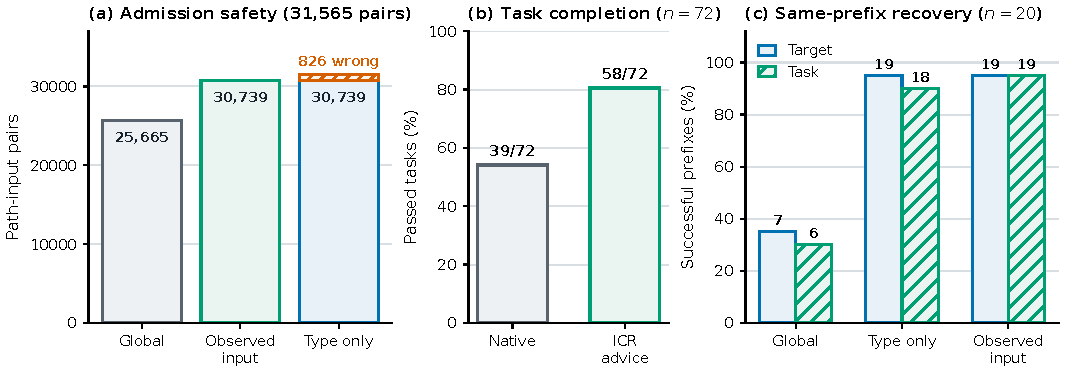
\includegraphics[width=.97\textwidth]{figures/results_overview.pdf}
\caption{PlanBench-XL results: (a) 31,565 path--input pairs; (b) 72 tasks; (c) 20 matched prefixes.}
\label{fig:results-overview}
\end{figure*}

\subsection{Observed-Input Certificate}
PlanBench-XL's independent retail executor yields 341 typed bypass paths
of two to five calls. Figure~\ref{fig:results-overview}(a) scores all 31,565
defined path--input pairs of the fixed read-only relation; here ``safe'' means
exact normalized output equality under the native executor on that snapshot.
The 9,250
failed-tool--input decisions below select at most one shortest route from
those pairs. The observed-input certificate recovers 5,074 safe
pairs inside the 59 paths rejected by global certification, without invoking
candidate paths at admission. Exhaustive native replay verifies every
classification. Among 9,250 failed-tool--input decisions, the shortest route
admitted by the observed-input certificate matches the native shortest-safe oracle in every case:
9,124 safe routes and 126 abstentions. Global certification finds 8,350
safe routes and abstains 900 times; type-only routing makes 126 wrong route
selections among these 9,250 decisions. The observed-input certificate thus recovers 774 safe decisions without
accepting the type-only errors.

\subsection{Native-Agent Recovery}
On 29 development first-failure prefixes, observed-input advice passes 26
continuations versus 20 for global advice (six paired gains, zero losses;
exact McNemar $p=0.031$). Four gains follow newly available packets. The
independent-task test below checks whole-trajectory transfer.

Table~\ref{tab:online-ablation} reports matched admission-rule controls: its
first row is whole-task pass and its second is trusted-target restoration
within 12 turns.
On the sealed 72-task seed-43 confirmation
(Fig.~\ref{fig:results-overview}(b)), ICR advice passes 58 tasks
versus 39 natively: 20 paired gains and one loss, a gain of 26.4 percentage
points (paired bootstrap 95\% interval [15.3, 37.5]; exact McNemar
$p=2.1\times10^{-5}$). Clustering by released reference path (49 groups)
and target datatype (19 groups) gives [16.1, 37.2] and [16.7, 35.5]
percentage-point intervals. Mean model requests differ by $-0.32$ per
task [$-3.99$, 3.32]. ICR emits 33 advice packets, and 17 of the 20 gains
contain a recovery event.
Across all 102 frozen eligible seed-43 tasks, including the 30-task diagnostic
stage, descriptive completion is 79/102 for ICR and 54/102 natively.

\begin{table}[t]
\centering\small\setlength{\tabcolsep}{4pt}
\caption{Matched PlanBench-XL online controls.}
\label{tab:online-ablation}
\begin{tabular}{ccccc}\toprule
\textbf{Frozen unit} & \textbf{Native} & \textbf{Global} & \textbf{Type only} & \textbf{ICR obs.}\\\midrule
21 tasks & 8/21 & \textbf{15/21} & \textbf{15/21} & \textbf{15/21}\\
20 prefixes & N/A & 7/20 & \textbf{19/20} & \textbf{19/20}\\
\bottomrule\end{tabular}
\end{table}

The prefix experiment starts from a native agent's already observed failed
state and isolates the three admission rules; it therefore has no separate
native continuation arm, shown as N/A in Table~\ref{tab:online-ablation}.

In the 21-task admission-rule holdout, global, type-only, and observed-input
advice emit 14, 15, and 15 packets, respectively. All 15 type-only packets in
this cohort pass the observed-input certificate, so the full-relation audit,
rather than this small task sample, exposes its 126 unsafe route decisions.
Of 62 frozen-order native captures, 26 met the
input-only failure rule; six formed the pilot and 20 the sealed same-prefix
confirmation (Fig.~\ref{fig:results-overview}(c)). Observed-input advice versus
global-certificate advice yields 12 paired local gains, no losses, a difference of 60 percentage
points (paired bootstrap 95\% interval [40, 80]; two-sided exact McNemar
$p=0.00049$). Whole-task success has 13 gains, no losses ($p=0.00024$).
Every local gain invokes a packet tool; four execute the full path. The
pilot enters neither test. In the ancillary type-only replay, all 20 first
paths coincide with and pass the observed-input certificate, yielding the
same local endpoint. Figure~\ref{fig:results-overview}(a) identifies the safety
distinction over the complete path--input relation.



\section{Related Work}
\textbf{Tool planning and recovery.}
ReAct and LLMCompiler establish model-led tool reasoning and program
execution~\cite{react,llmcompiler}; TaskBench and PlanBench-XL provide typed
workflows and path-preserving failure tests~\cite{taskbench,planbenchxl}.
HEART, ParaRecover, AgentTether, and AgentRewind address schema-guided recovery,
replanning, guarded actions, and rollback~\cite{heart,pararecover,agenttether,
agentrewind}. ICR instead resolves a concrete failed call by jointly selecting
replacement implementations and the least region that reconnects to the
continuation.

\textbf{Contracts and graph repair.}
Contract2Tool and ToolGate encode operation preconditions, effects, and
invocation guards~\cite{contract2tool,toolgate_published}; Atomic Task Graph,
counterfactual replay, DART, and REVISE structure tasks or repair execution
graphs~\cite{atg,gcjr,dart,revise}. Service reconfiguration addresses component
interfaces~\cite{servicereconfiguration}. ICR combines implementation and scope
optimization with observed-value binding; conditional equivalence and path-view
rewriting motivate its input-specific boundary-value certificate
~\cite{kawaguchi2010conditional,romero2020pathviews}.

For a fixed assignment, ICR closure is Horn-style implication reachability;
joint choice is a weighted constraint problem solved by tree DP or standard
variable elimination~\cite{dechter1999bucket}. The contribution is the repair
formulation that makes the reconnection boundary a decision variable and
composes it with observed-input value evidence. DART, REVISE, and AgentRewind
repair or roll back execution graphs, whereas Contract2Tool and ToolGate guard
individual calls; none of these abstractions jointly selects an implementation,
its least closed scope, and an input-specific relational witness.

\textbf{Execution authority and evaluation.}
Agent-First Tooling and transactional runtimes separate proposed from committed
effects~\cite{aft,cordon,mnemosyne2026}; provenance and AgentProp-Bench expose
authorization and parameter-propagation failures~\cite{pactprovenance,
agentprop}. ICR makes this boundary explicit: local interface and boundary-value
evidence determines admissibility, while grounded task context determines
authority to commit.


\section{Conclusion}
ICR combines interface-closed repair with observed-input value evidence.
On TaskBench, exact structural optimization finds minimum-cost repairs missed
by matched-information baselines. On the fixed PlanBench-XL relation, the
certificate expands safe route coverage without type-only errors. An executor-
backed replay composes joint scope selection with observed-input admission
while preserving unchanged downstream calls.
Observed-input advice restores the trusted target value at 19/20 input-only failure prefixes
versus 7/20 under global certification. The complete advice system improves
task completion from 39/72 to 58/72. These results show how explicit boundary
constraints and input-specific evidence support local recovery in read-only
agent workflows.


\balance
\bibliographystyle{IEEEtran}
\bibliography{IEEEabrv,references,continuation_references,repair_related_references,closure_related_references}
\end{document}
